\section{Theorie}
\label{sec:Theorie}
\subsection{Aufbau und Funktionsweise Geiger-Müller-Zählrohrs}
\label{subsec:theorie1}
Ein Geiger-Müller-Zählrohr besteht aus einem Kathodenzylinder und einer Drahtanode, die sich
innerhalb des Zylinders befindet. Die nachzuweisenden Teilchen treten durch ein Eintrittsfenster
aus einem dünnwandigen Material mit geringer Massenbelegung ein.
Der Aufbau des Zählrohrs ist in Abbildung \ref{fig:zaehlrohrskizze}
skizziert.

\begin{figure}
  \centering
  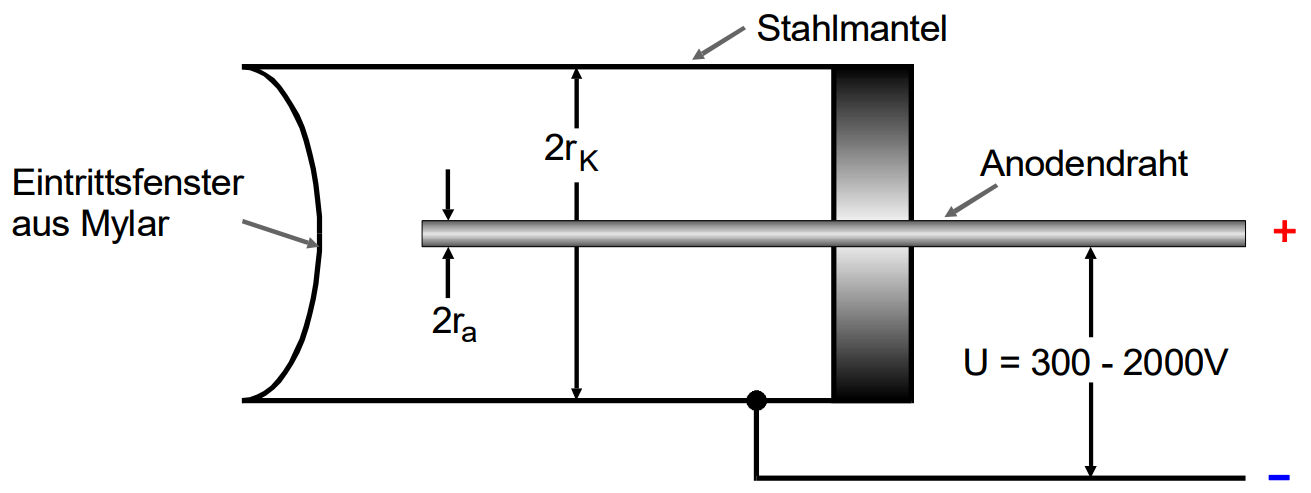
\includegraphics[width=\textwidth]{data/zaehlrohrskizze.png}
  \caption{Schematischer Aufbau eines Geiger-Müller-Zählrohrs,\cite{Versuchsanleitung}.}
  \label{fig:zaehlrohrskizze}
\end{figure}

Das Innere des Zählrohrs ist mit einem Gasgemisch befüllt, häufig besteht dieses aus einem Edelgas und einem Alkohol.
Dieses Gasgemisch kann von eintretender Strahlung ionisiert werden.
Es liegt eine Spannung $U$ zwischen Draht und Mantel an, sodass der Draht auf einem positiveren Potenzial als
der Mantel liegt. Daraus folgt, dass die durch die Ionisierung entstandenen Elektronen
eine Beschleunigung zum Draht hin erreichen. Falls die anliegende Spannung jedoch
zu gering ist, erreichen nur wenige bis keine Elektronen den Draht, da sie dann ausreichend
Zeit haben, mit den positiven Ionen des Gasgemisches zu rekombinieren.

Da die Energie der zu messenden ionisierenden Strahlung um Größenordnungen höher
ist als die Ionisierungsenergie des Gases, werden viele freie Elektronen durch ein eintretendes
Teilchen erzeugt. Es kann also angenommen werden, dass die Anzahl der Elektronen-Ionen-Paare
proportional zur Energie der eintretenden Strahlung ist. Die Abhängigkeit der Anzahl der Elektronen-Ionen-Paare
von der anliegenden Spannung kann ebenso untersucht werden, ein typischer
Verlauf dieser ist in Abbildung \ref{fig:nu} zu sehen.

\begin{figure}
  \centering
  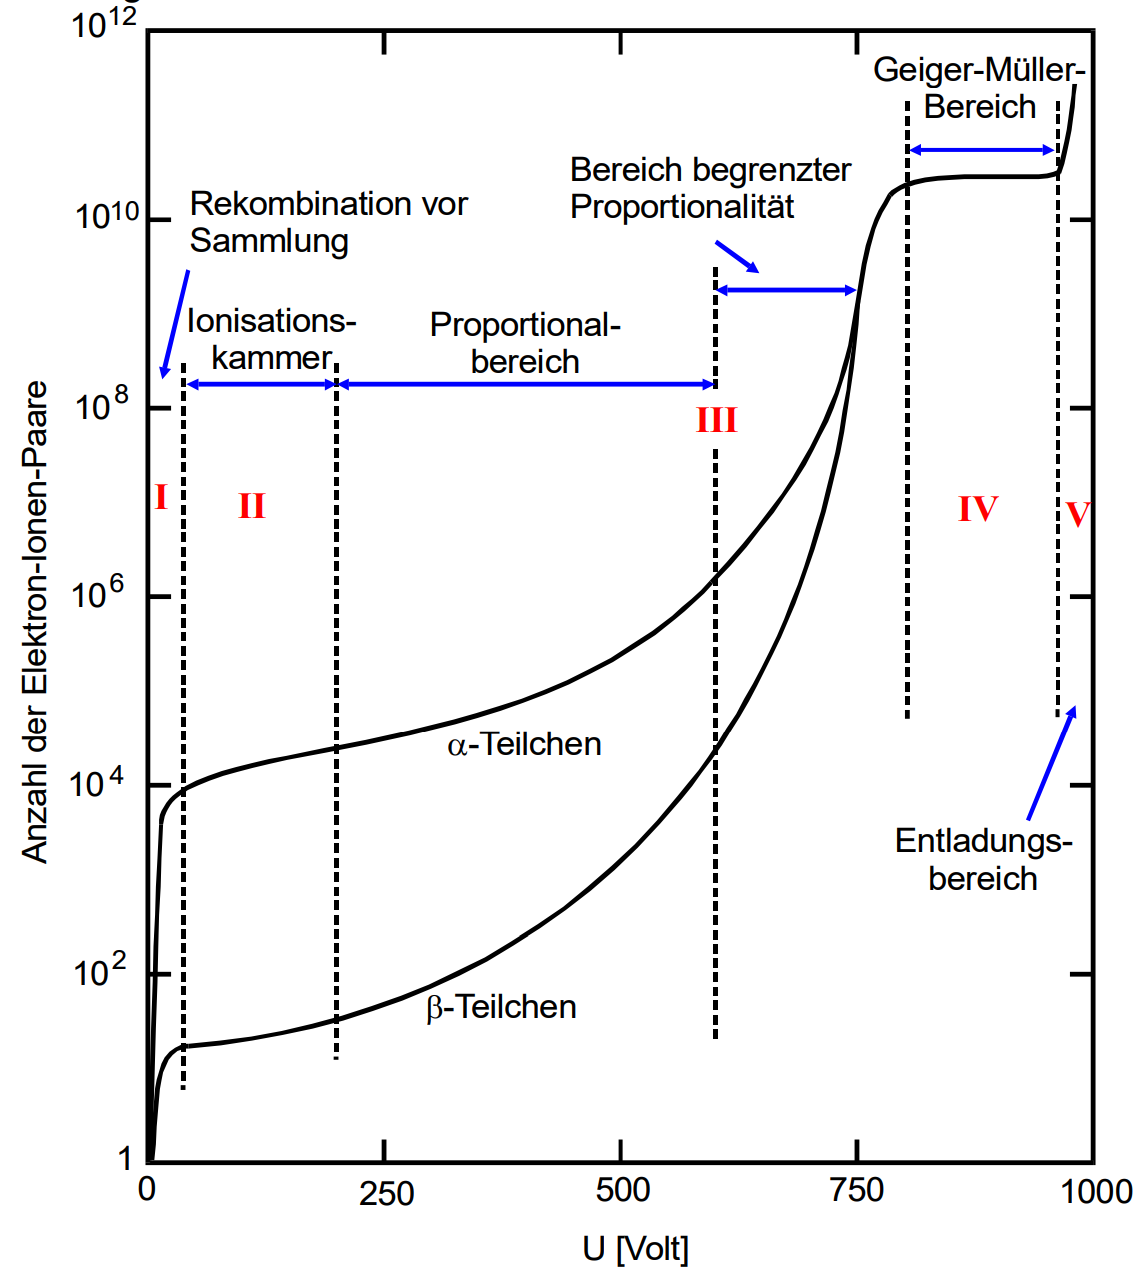
\includegraphics[width=\textwidth]{data/nu.png}
  \caption{Abhängigkeit der Anzahl der Elektronen-Ionen-Paare von der anliegenden Spannung,\cite{Versuchsanleitung}.}
  \label{fig:nu}
\end{figure}

Im Bereich I erreichen zunächst bei geringer Spannung fast keine Elektronen den Draht, da sie rekombinieren.
Wird die Spannung erhöht, erreichen immer mehr Elektonen den Draht, sodass ab einer gewissen Spannung
im Bereich II der Ionisationsstrom proportional zur Energie und Intensität der einfallenden Strahlung ist.
Erreichen die freigesetzten Elektronen ausreichend hohe Energien, um ihrerseits zu ionisieren,
dann wird das als Stoßionisation bezeichnet. Dieser Vorgang tritt bei einer weiteren Erhöhung der Spannung im Bereich III immer mehr auf.
Die Zahl der freien Elektronen nimmt lawinenartig zu, was als Townsend-Lawine bezeichnet wird.
Die Ladungsimpulse sind proportional zur Intensität und zur Energie der einfallenden Strahlung.\\
Im vierten Bereich, auch Auslösebereich genannt, breiten sich die Elektronenlawinen
im gesamten Zählrohr aus, da Photonen bei der Anregung der Gasatome durch Elektronenstoß entstehen.
Dies bewirkt, dass das Zählrohr nicht mehr zur Energiemessung eingesetzt werden kann. Auch können die
freigesetzten elektrischen Impulse in diesem Bereich mit wenig Aufwand gemessen werden, was vorher nicht unbedingt der Fall ist.

\subsection{Erklärung von Totzeit, Erholungszeit und Nachentladungen}
\label{subsec:theorie2}

Bei der Ionisation der Gasatome entstehen positiv geladene Ionen. Diese benötigen mehr Zeit,
um zum Mantel zu gelangen als die Elektronen zum Draht brauchen, da ihre Masse größer ist.
Für eine gewisse Zeit $T$ schirmt das Feld der Ionen das elektrische Feld nahe am Draht ab, sodass
Stoßionisation erschwert wird. Trifft dann ein Teilchen ein, kann dieses nicht detektiert werden.
Diese Zeit $T$ wird deswegen Totzeit genannt. Erst nach einer Zeit $T_\text{E}$ erreichen
die elektrischen Impulse ihre ursprüngliche Höhe, da erst dann die Ionen vollständig neutralisiert wurden.
Diese Zeit wird Erholungszeit genannt. Diese Zusammenhänge sind in Abbildung \ref{fig:qt}
dargestellt.

\begin{figure}
  \centering
  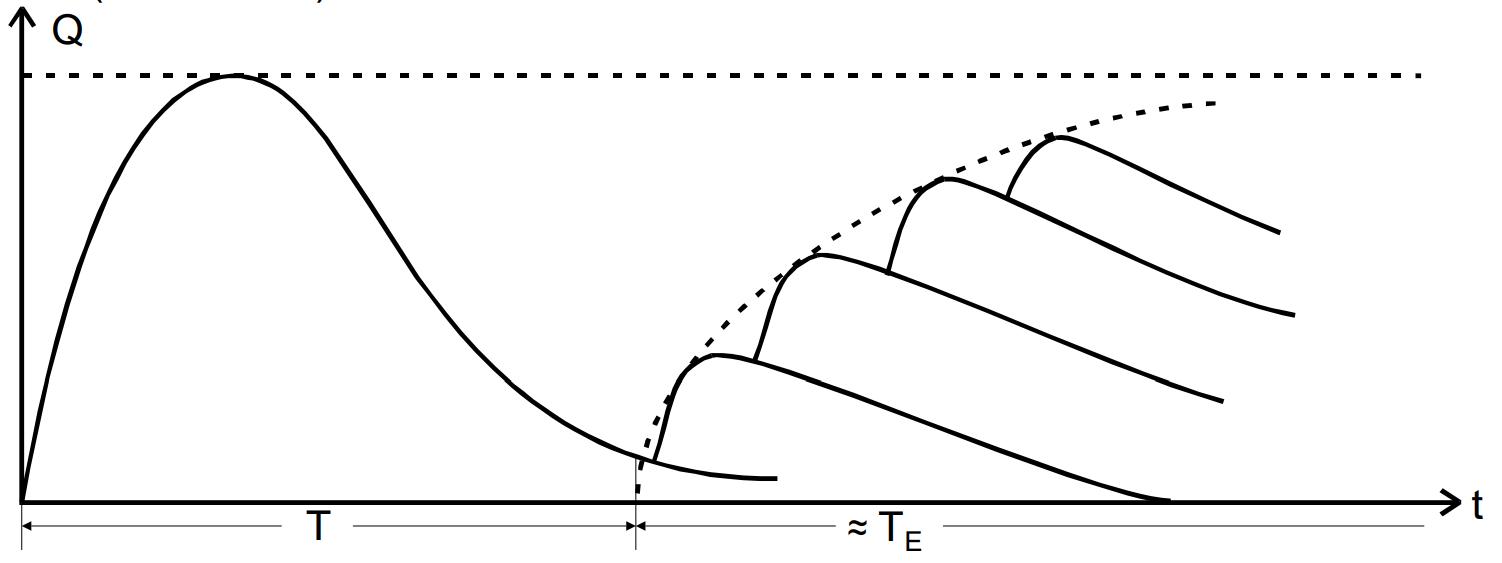
\includegraphics[width=\textwidth]{data/qt.png}
  \caption{Qualitativer Verlauf der gemessenen Ladung in Abhängigkeit der Zeit,\cite{Versuchsanleitung}.}
  \label{fig:qt}
\end{figure}

Eine Möglichkeit, die Totzeit experimentell zu bestimmen, ist die sogenannte
Zwei-Quellen-Methode, die in der Durchführung näher erklärt wird. Seien $N_1$ und $N_2$
Zählraten für zwei Strahler und $N_{1+2}$ die Zählrate, wenn beide Strahler gleichzeitig vermessen werden.
Dann beträgt die Totzeit
\begin{equation}
  T \approx \frac{N_1 + N_2 - N_{1+2}}{2N_{1+2}}\,.
  \label{eqn:zweiquellentotzeit}
\end{equation}\\
Beim Auftreffen der Ionen auf den Mantel könen Elektronen freigesetzt werden.
Die freigesetzten Elektronen können neue Lawinen auslösen und Nachentladungen zünden.
Dies ist nicht erwünscht, da ein einfallendes Teilchen mehrfach detektiert werden würde.
Dieser Effekt wird durch die Zugabe von Alkoholdämpfen zum Füllungsgas fast vollständig
unterdrückt, da die Gasionen die Alkoholmoleküle teilweise ionisieren und die Alkoholionen
beim Auftreffen auf den Mantel die freiwerdende Energie für Molekülschwingungen verwenden anstatt
weitere Elektronen aus dem Metall zu schlagen. Dadurch kann das unerwünschte mehrfache Zählung
fast vollständig vermieden werden.

\subsection{Charakteristik des Geiger-Müller-Zählrohrs}
\label{subsec:theorie3}

Die Charakteristik eines Zählrohrs ist der Verlauf der gemessen Teilchenzahl $N$ bei konstanter Intensität
der Strahlung in Abhängigkeit der anliegenden Spannung. Dies ist in Abbildung \ref{fig:charakteristik}
dargestellt.

\begin{figure}
  \centering
  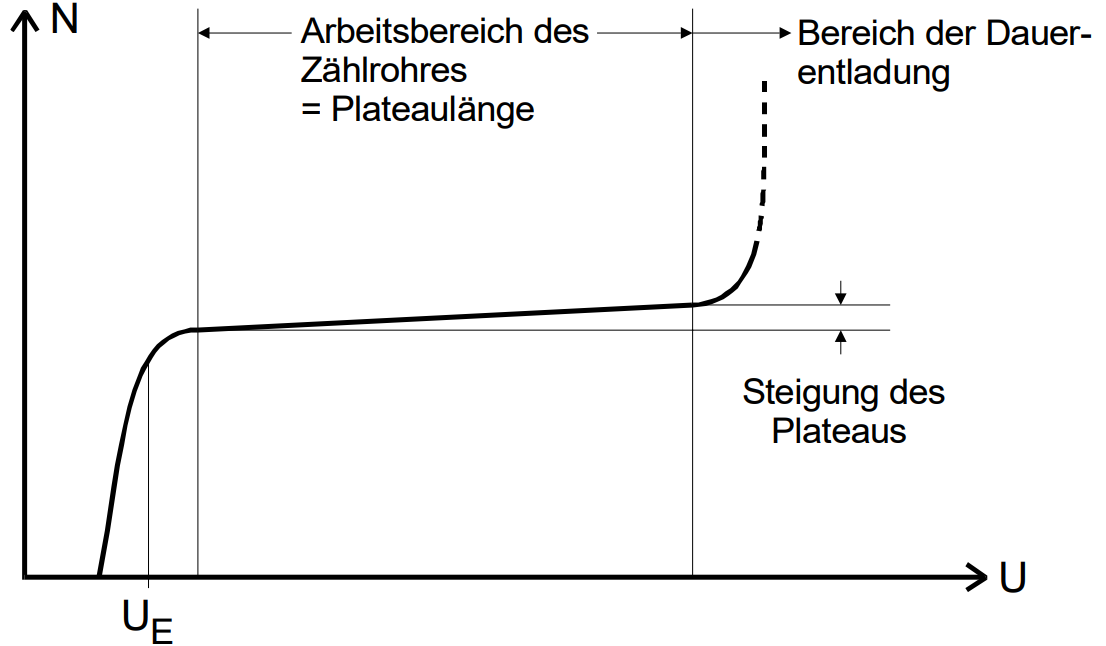
\includegraphics[width=\textwidth]{data/charakteristik.png}
  \caption{Auftragung der gemessenen Ereignisse in Abhängigkeit der anliegenden Spannung bei konstanter Strahlungsintensität,\cite{Versuchsanleitung}.}
  \label{fig:charakteristik}
\end{figure}

Der Auslösebereich beginnt etwa bei der Spannung $U_\text{E}$, dann folgt das sogenannte
Plateau. Bei einem idealen Zählrohr ist die Steigung des Plateaus null. In der Praxis
ist jedoch stets eine geringe Zunahme zu beobachten, da Nachentladungen trotz Zugabe
von Alkohol zum Gas nicht vollständig vermieden werden können. Eine kleine Steigung und ein
langes Plateau bedeutet eine hohe Qualität des Zählrohrs. Zum Ende des Plateaus hin
steigt die Zahl an Nachentladungen stark, sodass im Bereich der Dauerentladung bereits
ein ionisierendes Teilchen eine ständige Entladung zündet. Es resultieren hohe Stromdichten, die
das Zählrohr schnell zerstören.

\subsection{Zusammenhang zwischen Stromstärke und Ladungsmenge}
\label{subsec:theorie4}

Ist der mittlere Zählrohrstrom $\overline{I}$ bekannt, so lässt sich die Ladungsmenge
$\Delta Q$, die durch $Z$ Teilchen in der Zeit $\Delta t$ freigesetzt wird, mithilfe der Gleichung
\begin{equation}
  \overline{I} = \frac{\Delta Q}{\Delta t} Z
  \label{eqn:ladung}
\end{equation}
bestimmen.
